\chapter{Аналитическая часть}

В аналитическом разделе выдвигаются критерии, по которым можно классифицировать генетические алгоритмы. Проводится краткий обзор существующих генетических алгоритмов. Проводится классификация существующих методов
согласно выдвинутым критериям сравнения. Формализуется задача
в виде IDEF0–диаграммы.

\section{Анализ предметной области}

Транспортная сеть~---~совокупность транспортных линий, соединяющих узлы (города, предприятия, перекрёстки); практически представляется как граф с вершинами~---~узлами и дугами~---~линейными участками. В логистике под транспортной сетью понимают пространственную сеть, обеспечивающую движение транспорта или потока товара~\cite{shaitura2017distributed}. Существуют комплексные транспортные сети, объединяющие автодорожные, железнодорожные, воздушные и водные сети и связанную инфраструктуру.

Логистика охватывает планирование и управление потоками грузов и пассажиров, опираясь на транспортную сеть: в закупочной, производственной, распределительной и транспортной логистике оптимизируют перемещение ресурсов с учётом разных критериев, в том числе времени, стоимости и надёжности. 

\subsection{Основные определения}

\subsubsection{Задачи оптимизации}

В инженерных и прикладных задачах оптимизация рассматривается как процесс поиска такого состояния системы или конструкции, которое обеспечивает максимальное или минимальное значение заданной функции при фиксированных условиях~\cite{vereshchaga2023design}. 

Требуется найти вектор $\mathbf{x}^* = (x_1^*,\dots,x_j^*,\dots,x_n^*)^\intercal$, 
доставляющий минимум (максимум) функции $y = f(\mathbf{x})$ с заданной 
точностью $\varepsilon$, где $\mathbf{x} \in \mathbb{R}^n$.

Как правило, область допустимых значений D задаётся. Тогда задача формализуется целевой функцией в области допустимых значений D:
\begin{equation}
    f(\mathbf{x}) \to \min_{\mathbf{x} \in D}, \quad f(\mathbf{x}) \to \max_{\mathbf{x} \in D}
\end{equation}

Допустимым решением называется решение, удовлетворяющее всем ограничениям задачи, то есть принадлежащее множеству \(D\).

Многокритериальная оптимизация~(МКО)~---~это одновременная оптимизация минимум двух~(и более) конфликтующих между собой целевых функций в заданной области определения~\cite{khmelevski2024realestate}.

Окончательное решение принимает человек, которого принято называть лицом, принимающим решение~(ЛПР)~\cite{khmelevski2024realestate}. 

В общем виде постановка задачи МКО может быть представлена в виде \(\{D, f_1, \ldots, f_m\}\), где \(D\)~---~множество допустимых исходов, \(f_i\)~---~числовая функция, заданная на \(D\); при этом \(f_i(a)\) есть оценка исхода \(a \in D\) по \(i\)-му критерию~(\(i = 1, \ldots, m\))~\cite{khmelevski2024realestate}. Такая модель соответствует задаче принятия решений, в которой множество альтернатив соответствует множеству допустимых исходов, а оценочная структура задаётся вектором \((f_1, \ldots, f_m)\). Критерий \(f_i\) называется позитивным, если ЛПР стремится к его увеличению, и негативным, если ЛПР стремится к его уменьшению.

В задачах минимизации решение \(x_1\) доминирует над решением \(x_2\) (\(x_1~\prec~x_2\)), в случаях~\cite{polkovnikova2024evo}: 
\begin{enumerate}
	\item \(x_1\) не хуже \(x_2\) во всех целевых функциях;
	\item \(x_1\) строго лучше, чем \(x_2\) по крайней мере по одной целевой функции.
\end{enumerate}

Множеством Парето называется множество всех допустимых решений задачи многокритериальной оптимизации, которые не доминируются ни одним другим допустимым решением.

Фронт Парето~---~это множество всех векторных значений критериев, соответствующих решениям из множества Парето.

\subsection{Задачи поиска путей в графе}

Граф \(G\) состоит из двух множеств~---~множества вершин и множества рёбер, причём для каждого ребра указана пара вершин, которые это ребро соединяют. Вершины и рёбра называются элементами графа. 

Ориентированный граф \(G\) задаётся двумя множествами
\( G = (V, E), \)
где \(V\)~---~конечное множество, элементы которого называют вершинами (узлами); \(E\)~---~множество упорядоченных пар на \(V\) (подмножество \(V \times V\)), элементы которого называют дугами~\cite{belousov2025discrete}.

Если дуга \(e = (u, v)\), то говорят, что дуга \(e\) ведёт из вершины \(u\) в вершину \(v\), и обозначают это \(u \to v\)~\cite{belousov2025discrete}.

Путь в ориентированном графе \(G\)~---~это последовательность вершин~(конечная или бесконечная) \(
v_0, v_1, \ldots, v_n, \ldots\) такая, что \(v_i \to v_{i+1}\) для любого \(i\), если \(v_{i+1}\) существует~\cite{belousov2025discrete}.

Простой путь~---~это путь, все вершины которого, кроме, быть может, первой и последней, попарно различны~\cite{belousov2025discrete}.

Взвешенный граф~---~это граф, в котором каждому ребру присвоено числовое значение, называемое весом.

Однокритериальная задача поиска пути заключается в нахождении пути между двумя заданными вершинами взвешенного графа, при котором оптимизируется один скалярный критерий, обычно равный сумме весов рёбер на пути.

Векторная стоимость ребра~---~это обобщение понятия веса ребра во взвешенном графе, при котором каждому ребру сопоставляется вектор числовых значений, отражающих несколько критериев оценки (например, время, стоимость, надёжность). Каждому ребру
\(
v \in E
\)
ставится в соответствие вектор
\[
w(v) = \bigl(w_1(v), w_2(v), \ldots, w_m(v)\bigr),
\]
где каждая компонента соответствует отдельному критерию оптимальности.

Стоимость пути в пространстве критериев~---~это вектор, получаемый агрегированием векторных стоимостей всех рёбер, входящих в данный путь, и отражающий значения каждого критерия для всего пути в целом. Для пути
\[
P = \langle v_1, v_2, \ldots, v_k \rangle
\]
его стоимость определяется как
\[
W(P) = \sum_{i=1}^{k} w(v_i),
\]
где суммирование выполняется покомпонентно. Полученный вектор используется для сравнения путей на основе отношения доминирования или других правил многокритериального сравнения.

Нормализация и масштабирование критериев~---~это процедуры преобразования значений критериев к сопоставимому числовому масштабу, применяемые в многокритериальных задачах для устранения различий в размерностях и диапазонах значений. Нормализация обычно сводит значения критериев к безразмерному интервалу
\(
[0,1],
\)
тогда как масштабирование изменяет диапазон значений с сохранением относительных пропорций. 

\section{Формализация задачи}

Задача мультикритериального поиска путей в графе формально определяется как поиск множества Парето-оптимальных путей в ориентированном графе \(G(V,E)\) от стартовой вершины \(n_S \in V \) до конечной \(n_{End} \in V \), где каждый путь \(p_i=(n_S, \ldots, n_{End})\) имеет переменную длину \(K\) и оценивается по набору целевых функций \(\vec{f}(p)\), подлежащих минимизации~\cite{MARISTANYDELASCASAS2021105424}. Эта задача является обобщением классической задачи поиска кратчайшего пути и также известна в англоязычной литературе как Multi-Objective Shortest Path Problem~(MOSP Problem).

Следует отметить, что в зависимости от класса применяемых методов под решением
многокритериальной задачи поиска путей может пониматься либо точное построение
множества Парето-оптимальных путей, либо получение его аппроксимации. Точные методы
ориентированы на полное перечисление множества Парето, тогда как эвристические и
популяционные методы позволяют получить приближённое представление фронта Парето
при приемлемых вычислительных затратах.

Под компромиссным путём далее будет пониматься путь, который либо является Парето-оптимальным,
либо принадлежит аппроксимации множества Парето и не доминируется другими
допустимыми путями в рамках принятой точности аппроксимации.

Ниже представлена IDEF0-диаграмма решения задачи мультикритериального поиска путей в графе.
\begin{figure}[h!]
	\centering
	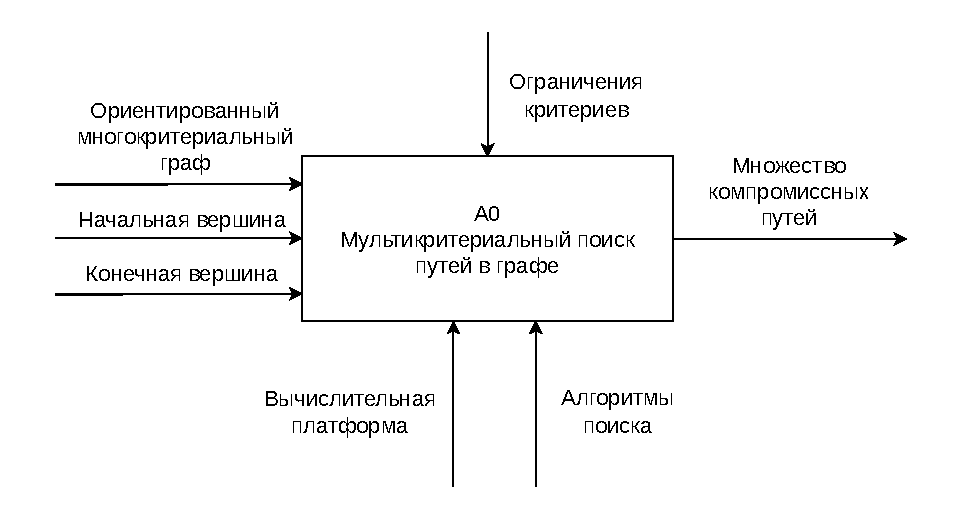
\includegraphics[width=0.7\textwidth]{inc/img/idef0.pdf}
	\caption{IDEF0-диаграмма решения задачи мультикритериального поиска путей в графе}
	\label{fig:idef0-task}
\end{figure}


\section{Основные методы}

\subsection{Методы скаляризации}

В задачах многокритериального поиска путей в графах методы скаляризации
применяются для сведения исходной векторной задачи оптимизации к
последовательности однокритериальных задач поиска пути. В качестве
допустимых решений рассматриваются пути в графе, соединяющие заданные
начальную и конечную вершины. Каждому пути $p$ ставится в соответствие
вектор значений частных критериев
$f(p) = (f_1(p), \ldots, f_m(p))$,
которые определяют показатели качества данного пути. Значения частных критериев $f_i(p)$ вычисляются путём агрегирования
стоимостей рёбер, входящих в рассматриваемый путь. Скаляризация заключается
в построении скалярной целевой функции $J(f(p))$, значения которой
используются для сравнения допустимых путей в рамках однокритериальной
задачи оптимизации.

В результате применения методов скаляризации исходная многокритериальная задача поиска путей сводится к однокритериальной задаче на графе. Для её
решения могут применяться классические алгоритмы поиска кратчайшего пути в графе или их модификации.

\subsubsection{Метод главного критерия}

Метод предполагает выбор одного функционала \(f_i(x)\) в качестве целевой функции. Остальные требования к результату, описываемые функционалами \(f_1,\) ... \(,f_m\),
учитываются с помощью введения необходимых дополнительных ограничений~\cite{avansky2007problems}. Тогда многокритериальная задача сводится к однокритериальной, вида:
\begin{equation}
	f_1(x) \to \max_{x \in D'},
	D' \subseteq D \subseteq \mathbb{R}^n, 
	D' = \{x \in D \mid f_i(x) \geqslant t_i,\; i = 2, \ldots, m\}.
\end{equation}
где \(D'\)~---~новое допустимое множество, \(t_i\) задают минимально допустимые уровни по второстепенным критериям. 

Подход требует обоснованного выбора <<главного>> критерия из многих.

\subsubsection{Линейная свёртка}

Данный метод позволяет заменить векторный критерий оптимальности \(f=(f_1,\) ... \(,f_m)\) на скалярный \(J\): \(D \to R\). Все частные целевые функционалы линейно объединяются в один скаляр с помощью весов \(\alpha_i\):
\begin{equation}
	J(x) = \sum_{i = 1}^{m} \alpha_i f_i(x) \to \max_{x \in D},
\end{equation}
где \(\alpha_i \geqslant 0\), а \(\sum_{i = 1}^{m} \alpha_i = 1\).

Весовые коэффициенты \(i\) могут при этом рассматриваться как показатели относительной значимости отдельных критериальных функционалов \(f_i\)~\cite{avansky2007problems}: чем важнее \(f_i\), тем больше должно быть \(\alpha_i\). 

\subsubsection{Максиминная свёртка}

В данном методе, в отличие от метода линейной свёртки, на целевой функционал \(J(x)\) оказывает влияние только тот
частный критерий оптимальности, которому в данной точке \(x\) соответствует наименьшее значение функции
\(f_i(x)\): 
\begin{equation}
	J(x) = \min f_i(x) \to \max_{x \in D}.
\end{equation}

Если в случае линейной свёртки, возможны <<плохие>> значения некоторых \(f_i\) за счёт достаточно <<хороших>> значений остальных целевых функционалов, то в случае максиминного критерия производится расчёт <<на наихудший случай>>~\cite{avansky2007problems}. Так, по значению \(J(x)\) можно определить гарантированную нижнюю оценку для
всех функционалов \(f_i(x)\). Этот факт расценивается как преимущество максиминного критерия перед методом
линейной свёртки~\cite{avansky2007problems}.

Следует отметить, что методы скаляризации в общем случае не позволяют получить
всё множество Парето-оптимальных путей. В зависимости от выбранной функции
свёртки и её параметров может быть найдено отдельное Парето-оптимальное решение
или компромиссный путь, обеспечивающий приемлемое соотношение между критериями.

\subsection{Точные методы}

Точные методы вычисляют полное множество Парето-оптимальных путей, обеспечивая получение всех недоминируемых решений. Их основной практический предел связан с тем, что количество таких путей может расти экспоненциально даже на графах умеренного размера~\cite{paixao2007, euler2024}.

\subsubsection{Меточные методы}

Основная идея меточных методов состоит в последовательном 
построении и обновлении множества недоминируемых промежуточных путей, каждый из которых 
представлен меткой, содержащей вектор значений критериев. В отличие от однокритериального случая, 
где каждой вершине соответствует единственная метка, многокритериальная постановка приводит 
к необходимости хранения множества недоминируемых меток, каждая из которых описывает отдельный уникальный недоминируемый путь.

В зависимости от того, к какому элементу графа привязывается метка, различают два класса методов: вершинно-меточные и дугово-меточные. В вершинно-меточных методах метка 
ассоциируется с вершиной графа и представляет состояние пути при достижении этой вершины. 
В дугово-меточных методах метка привязывается к состоянию пути непосредственно после прохождения 
определённой дуги, а обновление метки осуществляется посредством применения дуговой функции 
расширения при добавлении очередной дуги к частичному пути.

В обоих классах методов на каждой итерации выбирается 
необработанная метка, выполняется расширение соответствующего подпути, формируются новые метки 
и проводится проверка доминирования. Метка сохраняется для дальнейшего расширения, если она 
не доминируется существующими метками для того же состояния пути, а все доминируемые метки 
удаляются. Процесс продолжается до тех пор, пока множество необработанных меток не станет пустым, 
что гарантирует построение полного множества недоминируемых путей. В зависимости от стратегии 
выбора меток выделяют метко-установочные и метко-исправляющие алгоритмы, применимые как в 
вершинной, так и в дуговой формулировке~\cite{paixao2007,euler2024}:

\begin{itemize}
    \item Метко-установочные~(label-setting): метки сканируются таким образом, что хотя бы одна метка становится финальной, означая, что наилучший путь из \(s\) в определённую вершину найден. Для этой техники требуется гарантировать, что выбранная метка может стать окончательно недоминируемой;
    \item Метко-исправляющие~(label-correcting): любая метка может обновляться до тех пор, пока не выполнится условие остановки.
\end{itemize}

\subsubsection{Методы ветвей и границ}

Методы ветвей и границ~(branch-and-bound) для многокритериальной оптимизации основаны на поэтапном разбиении
исходной задачи на подзадачи и оценке их границ. В многокритериальной версии метода каждая подзадача сопровождается нижней оценкой, отражающей достижимые значения
критериев, и набором найденных недоминируемых решений, используемых в качестве верхней границы.
Подзадача исключается из рассмотрения, если при учёте наложенных ограничений в ней не существует ни одного допустимого решения,
если её нижняя оценка совпадает с найденным решением или если она полностью доминируется
текущим множеством недоминируемых точек~\cite{bauss2023}.

Алгоритм многокритериального метода ветвей и границ работает итеративно. На каждом шаге выбирается подзадача для обработки
в соответствии со стратегией выбора. После этого для выбранной подзадачи вычисляется нижняя
оценка. Если на этапе вычисления обнаружено допустимое решение, оно сравнивается с текущим
множеством найденных решений и, при необходимости, обновляет его. Определяется, подлежит
ли подзадача отсечению. Если отсечение невозможно, выполняется ветвление: исходная подзадача
разбивается на две новые, каждая из которых добавляется в список необработанных подзадач.
Процесс повторяется до тех пор, пока все подзадачи не будут обработаны или отброшены.

\subsection{Метаэвристические методы}

Метаэвристические методы предназначены для получения приближённого множества Парето-оптимальных путей при ограниченных вычислительных ресурсах. В отличие от точных методов, они не гарантируют нахождения всего множества Парето, однако способны эффективно работать на графах большой размерности и обеспечивать разнообразие найденных решений~\cite{PangilinanJanssens2007}.

\subsubsection{Эволюционные алгоритмы}

Эволюционные алгоритмы представляют собой класс стохастических методов поиска, вдохновлённых идеями естественного отбора и генетики. В этих алгоритмах используется популяция решений, каждое из которых кодирует допустимую точку пространства поиска~(в рассматриваемой задаче~---~путь в графе).

Классический эволюционный алгоритм включает следующие этапы~\cite{PangilinanJanssens2007}:
\begin{enumerate}
\item генерация начальной популяции;
\item оценка качества особей;
\item отбор родительских решений;
\item применение операторов вариации~(скрещивания и мутации);
\item формирование новой популяции.
\end{enumerate}

В эволюционных алгоритмах поддерживается множество потенциальных решений, для которых на каждой итерации проводится оценка качества. Однако в многокритериальных задачах качество решения не может быть выражено одним скалярным показателем. Вместо этого рассматривается множество недоминируемых решений~\cite{PangilinanJanssens2007}. Поэтому используется отношение доминирования по Парето, а целью эволюционного алгоритма является приближение множества Парето-оптимальных путей.

Для эволюционных алгоритмов над маршрутами естественными являются следующие типы операторов:
\begin{itemize}
\item мутация: локальное изменение пути, например вставка новой вершины, замена части маршрута альтернативным подмаршрутом, удаление циклов;
\item скрещивание: обмен подмаршрутами между двумя родительскими путями при условии сохранения связности и допустимости результата.
\end{itemize}

Показано~\cite{Horoba2009}, что простой эволюционный алгоритм, применённый к многокритериальной задаче кратчайшего пути, может обладать строгими аппроксимационными гарантиями: он обеспечивает построение приближённого множества Парето за полиномиальное время относительно размера входных данных.

\subsubsection{Методы роя частиц}

Методы роя частиц относятся к популяционным метаэвристикам и основаны на идее коллективного поведения групп организмов, таких как стаи птиц или косяки рыб. В исходной версии алгоритм был предложен Кеннеди и Эберхартом в 1995 году~\cite{vereshchaga2023design}.

В рассматриваемой задаче каждая частица представляет собой допустимый маршрут в графе. Для частицы вычисляется вектор значений критериев, отражающий качество маршрута. Сравнение решений выполняется с помощью отношения доминирования по Парето.

Алгоритм поддерживает популяцию частиц и внешний архив недоминируемых решений. Архив служит ориентиром для поиска, поскольку в многокритериальной задаче отсутствует единственное оптимальное решение. Каждая частица также запоминает своё личное лучшее состояние.

Положение частиц обновляется через дискретные изменения маршрутов, направленные на приближение к личному лучшему решению и выбранному элементу архива. После изменения маршруты корректируются, чтобы оставаться допустимыми (например, удаляются циклы). Далее новые решения сравниваются с архивом: доминируемые исключаются, недоминируемые добавляются. Если архив становится слишком большим, из него удаляют решения из областей с высокой плотностью, чтобы сохранять равномерное представление фронта Парето.

На выходе алгоритм формирует множество недоминируемых маршрутов, которое является приближением множества Парето для многокритериальной задачи поиска пути.

\section{Сравнение основных методов}

Для сравнения групп методов, рассмотренных ранее, выделены следующие критерии:

\begin{enumerate}
    \item Доступность: способность метода корректно находить Парето-оптимальные пути в невыпуклых областях фронта Парето.
    \item Точность: способность получать точные Парето-оптимальные решения.
    \item Полнота: способность метода получать полное множество Парето-оптимальных путей.
    \item Вычислительная сложность.
\end{enumerate}

\begin{table}[h]
\centering
\caption{Сравнение групп методов решения многокритериальной задачи поиска путей}
\label{tab:comparison_methods}


\begin{tabular}{|m{3.1cm}|>{\centering\arraybackslash}m{3.3cm}|
>{\centering\arraybackslash}m{2.3cm}|
>{\centering\arraybackslash}m{2.1cm}|
>{\centering\arraybackslash}m{4cm}|}

\hline
\textbf{Методы} 
& \textbf{Доступность} 
& \textbf{Точность} 
& \textbf{Полнота}
& \textbf{Вычислительная сложность} \\ \hline

\makecell[l]{Методы\\скаляризации}
& $+/-$
& $-$
& $-$
& \makecell{Полиномиальная\\\cite{article}} \\ \hline

\makecell[l]{Точные\\методы}
& $+$ 
& $+$ 
& $+$
& \makecell{Экспоненциальная\\\cite{euler2024}} \\ \hline

\makecell[l]{Метаэвристи-\\ческие\\методы}
& $+$ 
& $-$ 
& $-$
& \makecell{Полиномиальная\\\cite{May2023ACOReport, BianQian2022NSGAII}} \\ \hline

\end{tabular}
\end{table}

На основе таблицы можно сформулировать следующие выводы:

\begin{enumerate}[label=---]
    \item Методы скаляризации характеризуются низкой вычислительной сложностью и обеспечивают высокую доступность решений при выпуклом фронте Парето, однако не позволяют корректно восстанавливать невыпуклые области, не обеспечивают точности в таких случаях и не гарантируют полноты множества Парето-оптимальных путей.
    
    \item Точные методы обладают максимальной доступностью, обеспечивают получение полностью корректного и полного множества Парето-оптимальных путей с высокой точностью, но их практическое применение существенно ограничено экспоненциальной вычислительной сложностью, обусловленной ростом количества недоминируемых меток.
    
    \item Метаэвристические методы демонстрируют высокую доступность и способны находить решения в невыпуклых областях фронта Парето, однако предоставляют только приближённые результаты, не обеспечивают точности и не гарантируют полноты множества Парето-оптимальных путей, несмотря на полиномиальную вычислительную сложность.
\end{enumerate}

\section*{Вывод}

В данном разделе были выдвинуты критерии классификации генетических алгоритмов. Проведен краткий обзор существующих методов, а также их классификация согласно выдвинутым критериям сравнения. Была формализована задача в виде IDEF0–диаграммы.
